\documentclass[12pt]{article}
\usepackage[utf8]{inputenc}
\usepackage{amsmath}
\usepackage{color,lineno,setspace,multirow}
\usepackage{graphicx}
\usepackage[top=2.4cm,left=2.4cm,top=2.4cm,bottom=2.4cm,includefoot]{geometry}
\usepackage{natbib}
\usepackage{caption}
\usepackage{pdflscape}

\bibliographystyle{bes}

\begin{document}

\linenumbers
\modulolinenumbers[1]

\textbf{Title:} Bringing Elton and Grinnell together: a quantitative framework to represent the biogeography of ecological interaction networks

\textbf{Authors:} Dominique Gravel$^{1,2,*}$, Benjamin Baiser$^{3}$, Jennifer A. Dunne$^{4}$, Jens-Peter Kopelke$^{5}$, Neo
Martinez$^{6}$, Tommi Nyman$^{7}$, Timoth\'ee Poisot$^{2,8}$, Spencer A. Wood$^{9}$, Daniel B. Stouffer$^{10}$, Jason M. Tylianakis$^{10,11}$ Tomas Roslin$^{12}$,\\

1: Canada Research Chair in Integrative Ecology. D\'epartement de
biologie, Universit\'e de Sherbrooke, 2500 Boulevard l'Universit\'e,
Sherbrooke (Québec). J1K 2R1\\

2: Qu\'ebec Centre for Biodiversity Sciences\\

3: University of Florida, Department of Wildlife Ecology and Conservation, 110 Newins-Ziegler Hall, PO Box 110430, Gainesville, Fl. 32611-0430 \\

4: Santa Fe Institute, 1399 Hyde Park Road, Santa Fe, NM 87501, USA.\\

5: Senckenberg Research Institute and Natural History Museum, Senckenberganlage 25, D-60325 Frankfurt am Main, Germany\\

6: Ecology and Evolutionary Biology Department, University of Arizona, P.O. Box 210088, Tucson, AZ 85721, USA\\

7: University of Eastern Finland, Department of Environmental and Biological Sciences, P.O. Box 111, FI-80101 Joensuu, Finland\\

8: Université de Montréal, Département des Sciences Biologiques, 90 Avenue Vincent d’Indy, Montréal, QC H2V3S9, Canada.\\

9: University of Washington, School of Environmental and Forest Sciences,
Box 352100, Seattle, WA 98195, USA\\

10: Centre for Integrative Ecology, School of Biological Sciences, University of Canterbury, Private Bag 4800, Christchurch, New Zealand\\

11: Department of Life Sciences, Imperial College London, Silwood Park Campus, 
Buckhurst Road, Ascot, Berkshire SL5 7PY, United Kingdom\\

12: Department of Ecology, Swedish University of Agricultural Sciences, Box 7044, 750 07 Uppsala, Sweden\\

\textbf{Keywords:} networks, spatial ecology, co-occurrence, probability of interaction\\

\textbf{Words in the abstract:}

\textbf{Words in the main text:}

\textbf{Words in the legends:}

\textbf{Figures: 6}

\textbf{Tables: 2}

\textbf{References:}

\newpage
\doublespacing

%=============================================================================%
\section*{Abstract}

Biogeography has traditionally focused on the spatial distribution and
abundance of species. Both are driven by the way species interact with one
another, but also by the way these interactions vary across time and space.
Here, we call for an integrated approach in which community structure
represented as a network of ecological interactions, and show how it
translates to biogeography questions. We propose that the ecological niche may
be redefined to encompass the effect of the environment on species
distribution (the Grinnellian dimension of the niche) and on the ecological
interactions among them (the Eltonian dimension). Starting from this 
concept, we develop a quantitative theory to explain turnover of interactions
in space and time -– \emph{i.e.} a novel approach to interaction distribution
modelling. We apply this framework to host–parasite interactions across Europe
and find that two aspects of the environment (temperature and precipitation)
exert a strong imprint on species co-occurrence, but not on species
interactions. Even where species co-occur, interaction proves to be stochastic
rather than deterministic, adding to variation in realized network structure.
We also find that a large majority of host-parasite pairs are never found
together, thus precluding any inferences regarding their probability to
interact. This first attempt to explain variation of network
structure at large spatial scales opens new perspectives at the interface
of species distribution modelling and community ecology.

\newpage

%=============================================================================%
\section*{Introduction}

Community ecology is \textit{the study of the interactions that determine
the distribution and abundance of organisms} \citep{Krebs2001}. Despite a
general consensus on this definition (Scheiner2007), research on variation in
community structure has mostly focused on the spatial and temporal turnover
of species composition \citep{Anderson2011}, neglecting variation in the way
species interact with each other, despite accumulating empirical evidence that
this is a major source of diversity \citep{Poisot2015a}. Given this omission,
it is perhaps not surprising that biogeographers are still struggling to
establish whether interactions actually impact the distribution of species at
large spatial scales \citep{Wisz2012, Kissling2012}: treating interactions
as fixed events neglects a large part of the complexity of empirical
communities, and will most likely deliver underwhelming results. Recent
attempts at accounting for interactions in species distribution models
\citep{Pollock2014, Pelissier2013} have brought some methodological advances,
but are not sufficient for two reasons. First, these techniques are still
based on a `species-based' approach to communities, where interactions
are merely treated as fixed covariates affecting distribution. Second,
they failed to provide a conceptual step forward, both in their treatment
of interactions and in the quality of the predictions they make.

Because it is an explicit description of species interactions, network
approaches offer a convenient representation of communities. Species are
represented as nodes, so that networks already encompass all the information
used by current approaches; in addition, interactions are represented by
links, so that networks provide additional, higher-order information on
community structure. To date, studies of network diversity have mostly been
concerned with the distribution of interactions within locations, and less so
with variation among locations \citep{Dunne2005, Bascompte2007, Ings2007,
Kefi2012}. There is, however, ample evidence that interaction networks vary in
space and time \citep{Laliberte2010, Poisot2012, Albouy2014, Poisot2016,
Trojelsgaard2015}, even though there is no common framework with which to
generalize these results. Metacommunity theory provides explanations for
variation in the distribution of the nodes \citep{Gravel2011c, Pillai2011},
but there is no such explanation to the variation of node and link
occurrences. Consequently, we urgently need a conceptual framework to
formalize these observations, as it is the only way towards fulfilling the
goal of community ecology: providing cogent predictions about, and
understanding of, the structure of ecological communities.

Given the historically different approaches to modelling the distributions of
species vs. interactions, there is a clear need to bring the two together.
Here, we offer an integrated approach to do so, adopting the view that
community structure is best represented as a network of ecological
interactions. Based on this idea, we propose a new description of the basic
concept of the ecological niche that integrates the effect of the environment
on species distribution and on the ecological interactions among them.
Starting from this redefined concept, we develop a quantitative theory to
explain turnover of interactions in space and time. We first present the
conceptual framework, and then formalize it mathematically, using a
probabilistic model to represent the sampling of the regional pool of
interactions. At the level of species pairs, the statistical approach could be
conceived as an interaction distribution model. At the community level, the
approach provides a likelihood-based method to compare different hypotheses of
network turnover. As an illustrative example, we apply this novel framework to
a large data set on host–parasite interactions across Europe and perform test
hypotheses underlying variation of species and interactions. The network
structure changes systematically across the latitudinal gradient, with a peak
of connectance at intermediate latitudes.

%=============================================================================%
\section*{The two dimensions of community structure}

The problem of community assembly is often formulated as \textit{how are
species sampled from a regional pool to constitute a local community
\citep{Gotzenberger2012}?} This question could be rewritten to address the
problem of network assembly, as \textit{how do samples from a regional pool of
interactions constitute a local interaction network?} An illustration of this
problem for a food web is provided in Fig. 1. The regional pool of
interactions, or \emph{metaweb}, represents potential interactions among all
species that could be found in a given area. In this particular case, there
are 275 nodes, and 1173 links among the plants (52 nodes), herbivores (96
nodes), and parasitoids (127 nodes) from Northern Europe. An instance of a
local community is also illustrated, with 45 nodes and 93 interactions. Only
55.0\% of all potential interactions (plant-herbivore or herbivore parasitoid
combinations) are realized locally, revealing the stochastic nature of
ecological interactions. Our objective here is to provide a conceptual
framework to explain the sampling of the regional pool of interactions, along
with a quantitative method to predict it. The problem could be formalized
sequentially by understanding first why only a fraction of the species co-
occur locally and second why these species do or do not interact.

There are multiple causes of spatial turnover of species co-occurrence. The first
and most-studied driver is the effect of variation in the abiotic environment
on species performance. Combined with specific responses in demography, it
generates variation among sites by selecting the locally fittest species
\citep{Leibold2004}. Stochasticity plays an additional role, either because
colonization and extinction events \citep{Hanski1999} are inherently
unpredictable or because strong non-linear feedbacks in community dynamics
generate alternative transients and equilibria \citep{Chase2007, Vellend2014}.
Analyses of community turnover are usually performed with data represented in
a table with rows corresponding to sites (or measurements) and columns to
species. Metrics of beta diversity quantify the variance of this community
data \citep{Legendre2005}. Traditional approaches rely on measures of
dissimilarity among communities, such as the Jaccard or Bray–Curtis indices.
More recent approaches decompose total variation of the community data into
species and site contributions to beta diversity \citep{Legendre2013}, and
further partition it into dissimilarity due to changes in species richness and
dissimilarity due to actual species turnover \citep{Baselga2010;
Carvalho2012}. Even though these methods compare whole lists of species among
sites or measurements, they remain fundamentally `species-based', since they
report variation within columns. None of them explicitly considers variation
of associations (i.e., of pairs or higher-order motifs –
\citealt{Stouffer2007}).

Similarly, we are getting a better understanding of interaction turnover. As
mentioned above, in the network approach to community structure, species and
interactions are represented by nodes and links, respectively. Associations
can also be represented by matrices in which entries represent the occurrence
or intensity of interactions among species (rows and columns). Network
complexity is then computed as the number of interactions (in the case of
binary networks) or interaction diversity (in the case of quantitative
networks, \citealt{Bersier2002}). Variability in community structure
consequently arises from the turnover of species composition, along with
turnover of interactions among pairs of species. The occurrence and intensity
of interactions could vary because of the environment, species abundance, and
higher-order interactions \citep{Poisot2015a}. Variation in community
composition can be independent of variation of ecological
interactions, suggesting that species and interaction distribution may well
respond to different drivers \citep{Poisot2012}.

The "niche" is by far the dominant concept invoked to explain species
distributions and community assembly, from the local to the global scale.
Following \citealt{Hutchinson1957}, the niche is viewed as the set of
environmental conditions allowing a population to establish and persist (see
also \citealt{Holt2009}). Community turnover arises as a result of successive
replacement of species along an environmental gradient, in agreement with the
Gleasonian view of communities \citep{Gleason1926}. The concept is
straightforward to put into practice with species distribution models, as it
maps naturally on available distributional and environmental data. Consequently, a vast array of statistical tools have been developed to
implement it (e.g. BIOMOD \citealt{Thuiller2003}, MaxEnt
\citealt{Phillips2006}). It is however much harder to account for ecological
interactions within this approach \citep{Peterson2011}. As such, these
interactions are often viewed as externalities constraining or expanding the
range of environmental conditions required for a species to maintain a viable
population \citep{Pulliam2000, Soberon2007, Boulangeat2012}.

Interestingly, the ecological network literature also has its own "niche
model" to position a species in a community \citep{Williams2000}. The niche of
a species in this context represents the multidimensional space of all of its
interactions. Each species is characterized by a niche position, an optimum
and a range over three to five different niche axes \citep{Williams2000, Eklof2013}.
The niche model of food web structure and its variants have successfully
explained the complexity of a variety of networks, from food webs to
plant–pollinator systems \citep{Allesina2008, Williams2010, Eklof2013}. This
conceptual framework is, however, limited to local communities, and does not
provide any explanation for the turnover of network structure along
environmental gradients.

%=============================================================================%
\section*{The integrated niche}

Despite several attempts to update the concept of the ecological niche,
ecologists have not moved far beyond the "n-dimensional hypervolume" defined
by Hutchinson. Despite its intuitive interpretation and easy translation into
species distribution models \citep{Boulangeat2012, Blonder2014}, the concept
has been frequently criticized \citep{Hardin1960, Peters1991, Silvertown2004},
and several attempts have been made to expand and improve it
\citep{Pulliam2000, Chase2003, Soberon2007, Holt2009, McInerny2012b}.

Part of the problem surrounding the niche concept has been clarified with the
distinction between Eltonian and Grinnellian definitions \citep{Chase2003}.
The Grinnellian dimension of the niche is the set of environmental conditions
required for a species to maintain a population in a location. The Grinnellian
niche is intuitive to apply, and constitutes the conceptual backbone of
species distribution models. The Eltonian niche, on the other hand, is the
effect of a species on its environment. While this aspect of the niche is well
known by community ecologists, it is trickier to turn into predictive models.
Nonetheless, the development of the niche model of food web structure
\citep{Williams2000} and its parameterization using functional traits
\citep{Gravel2013; Bartomeus2016} made it more operational.

These perspectives are rather orthogonal to each other, and this has resulted
in considerable confusion in the literature \citep{McInerny2012a}.
\citealt{Chase2003} attempted to reconcile with the following definition:
"[The niche is] the joint description of the environmental conditions that
allow a species to satisfy its minimum requirements so that the birth rate of
a local population is equal to or greater than its death rate along with the
set of per capita effects of that species on these environmental conditions".
Their representation merges zero-net-growth isoclines delimiting the
Grinnellian niche ("when does the population persists?"") with impact vectors
delimiting the Eltonian niche ("what is the per-capita impact?"). While this
representation has been very influential in local-scale community ecology (the
resource-ratio theory of coexistence, \citealt{Tilman1982}), it remains
impractical at larger spatial scales because of the difficulties in measuring
it. The absence of any mathematical representation of the niche that can be
easily fit to ecological data may explain why biogeographers are still
struggling to develop species distribution models that also consider
ecological interactions. Thus, a more integrative description of the niche
will be key to understand spatial and temporal turnover in community
structure.

We propose to integrate the two perspectives of the niche using a visual
representation of both components (Fig. 2). The underlying rationale is that,
in addition to the environmental constraints on demographic performance (Fig.2
top panel), any organism requires resources to meet its metabolic demands and
to sustain reproduction (Fig. 2 nodes in network of bottom panel). Abiotic
environmental axes are any non-consumable factors affecting the demographic
performance of an organism. Alternatively, the resource axes are traits of the
resources that allow interactions with the consumer. The niche can therefore
be viewed as the set of abiotic environmental variables (the Grinnellian
component) along with the set of traits (the Eltonian component) that allow a
population to establish and to persist at a location. Accordingly, each
species can be characterized by an optimal position along both the
environmental (x-axis) and the trait (y-axis) plane. The integrated niche is
then the hypervolume where interactions can occur and sustain a population.

This approach radically changes the representation of the niche, putting species
distributions and ecological interactions into the same formalism.
Moreover, it allows the limits of the niche axes to be independent of each other (as in the
example in Fig. 2), or to interact. For instance, the optimal
prey size for predatory fishes could decline with increasing temperature
\citep{Lelong2015}, which would make diet boundaries functions of the
environment. Alternatively, we could also consider that the growth rate
of the predator changes with the size of its prey items, thereby altering the
environmental boundaries.

%========================================================%
\section*{A probabilistic representation of interaction networks in space}

We now formalize the integrated niche with a probabilistic approach to
interactions and distributions. In particular, we seek to represent the
probability that an interaction between species $i$ and $j$ occurs at location
$y$. We define $L_{ijy}$ as a stochastic variable, and focus on the
probability that this event occurs, $P(L_{ijy})$. We note that the occurrence
of an interaction is dependent on the co-occurrence of species $i$ and $j$.
This argument might seem trivial at first, but the explicit consideration of
this condition in the probabilistic representation of ecological interactions
will prove instrumental to understanding their variation. We define $X_{iy}$
as a stochastic variable representing the occurrence of species $i$ at
location $y$. The quantity we seek to understand is the probability of a joint
event, conditional on the set of environmental conditions $E_y$:

%-----------------
\begin{equation}
	\text{P}(X_{iy},X_{jy},L_{ijy}|E_y)
\end{equation}
%-----------------

Or simply said, the probability of observing both species $i$ and $j$ plus an
interaction between $i$ and $j$ given the conditions $E_y$ at location $y$.
This probability could be decomposed into two parts using the product rule of
probabilities:

%-----------------
\begin{equation}
	P(X_{iy},X_{jy},L_{ijy}|E_y)=P(X_{iy},X_{jy}|E_y)P(L_{ijy}|X_{iy},X_{jy},E_y)
\end{equation}
%-----------------

The first term on the right-hand side of the equation is the probability
of observing the two species co-occurring at location $y$. It corresponds
to the Grinnellian dimension of the niche. The second term represents the
probability that an interaction occurs between species $i$ and $j$, given that
they are co-occurring. This predicate can be refined using information on
trait distribution and trait matching rules (\citep{Bartomeus2016}).
Above, we referred to this entity as the "metaweb" and it corresponds to
the Eltonian dimension of the niche. Below, we will see how this formalism
can be directly fit to empirical data. But before turning to an application,
we will discuss the interpretation of different variants of these two terms.

\subsection*{Variants of co-occurrence}

There are several variants to the co-occurrence probability, representing
different hypotheses concerning temporal and spatial variation in network structure
(see the explicit formulations in Table 1). The simplest model relates the
probability of co-occurrence directly to the environment, $P(X_{iy},X_{jy}|E_y)$.
In this situation, there are no underlying assumptions about the ecological
processes responsible for co-occurrence. It could arise because interactions
constrain distribution \citep{Pollock2014, Cazelles2016} or,
alternatively, because of environmental requirements shared between $i$ and
$j$. In the former case, species are not independent of each other and the
conditional occurrence must be accounted for explicitly, $P(X_{iy},X_{jy}
|E_y)=P(X_{iy}|E_y,X_{jy})P(X_{jy}|E_y)$. In the latter case, species are
independent, and only the marginal occurrence must be accounted for, $P(
X_{ijy}}|E_y)=P(X_{iy} |E_y)P(X_{jy} |E_y)$.

The co-occurrence probability itself could depend on ecological interactions.
This should be viewed as the realized component of the niche (i.e. the
distribution when accounting for species interactions). Direct pairwise
interactions such as competition, facilitation, and predation have long been
studied for their impact on co-distribution (e.g. \citealt{Diamond1976,
Connor1980, Gotelli2000}). Second- and higher-order interactions (e.g. trophic
cascades) could also affect co-occurrence. Co-occurrence of multiple species
embedded in ecological networks is a topic of its own, however, and is
influenced by both network topology and species richness \citep{Cazelles2016}.
Not only direct interactions influence co-occurrence, but indirect
interactions do as well (e.g. plant species sharing an herbivore, or
herbivores sharing parasitoids, could repel each other in space
\citealt{Holt1993}). The impact of direct interactions and first-order
indirect interactions on co-occurrence tends to vanish with increasing species
richness in the community. Further, co-occurrence is also influenced by the
covariance of interacting species to an environmental gradient
\citep{Cazelles2015}. Because of the complexity of relating co-occurrence to
the structure of interaction networks, we will focus here on the variation of
interactions and not on their distribution, and leave this specific issue for
the Perspectives section and future research.

\subsection*{Variants of the metaweb}

There are also variants of the metaweb. First, most documented metawebs have
thus far considered ecological interactions to be deterministic, rather than
probabilistic (e.g. \citealt{Havens1992, Wood2015}). Species are assumed to
interact whenever they are found together in a location, independent of their
local abundance and the local environment. In other words,
$P(L_{ijy}|X_{ijy}=1) = 1$ and $P(L_{ijy}|X_{ijy}=0) = 0$. This approach might
be a reasonable approximation if the spatial or temporal scale of sampling and inference is so
large that the probability of observing at least one interaction converges to
unity. In this scenario, network variation arises solely from species
distributions.

Second, ecological interactions could also vary with the environment, so that
$P(L_{ijy} |E_y)$. Although it is rare to see a conditional representation of
pairwise ecological interactions, experimental studies have frequently
revealed interactions to  be sensitive to the environment. For instance,
\citep{Mckinnon2010} showed that predation risks of shorebirds vary at the
continental scale, decreasing from the south to the north. It is also common
to see increasing top-down control with temperature (e.g. \citealt{Shurin2012,
Gray2016}). Effects of the environment on interactions also propagate up the
community and influence network structure \citep{Tylianakis2007, Woodward2010;
Petchey2010; Lelong2015}.

%========================================================%

\section*{Application: continental-scale variation of host-parasite community structure}

We now turn to an illustration of our framework with the analysis of an
empirical dataset of host–parasite networks sampled throughout the south–north
environmental gradient in continental Europe. The focal system consists of
local food webs of willows (genus Salix), their galling insects, and the
natural enemies (parasitoids and inquilines) of these gallers. Targeting this
system, we ask: i) how much does network structure vary across the gradient,
and ii) what is the primary driver of network turnover across the gradient?

\subsection*{Data}

Communities of willows, gallers, and parasitoids are species-rich and
widely distributed, with pronounced variation in community composition across
space. The genus Salix includes over 400 species, most of which are shrubs or
small trees \citep{Argus1997}, and is common in most habitats across the
Northern Hemisphere \citep{Skvortsov1999}. Willows support a highly diverse
community of herbivorous insects, with one of the main herbivore groups being
gall-inducing sawflies (Hymenoptera: Tenthredinidae: Nematinae: Euurina
\citep{Kopelke1999}). Gall formation is induced by sawfly females during
oviposition, and includes marked manipulation of host-plant chemistry by the
galler \citep{Nyman2000}. The enemy community of the gallers includes nearly
100 species belonging to 17 insect families of four orders
\citep{Kopelke2000}. These encompass two main types: inquiline larvae
(Coleoptera, Lepidoptera, Diptera, and Hymenoptera) feed primarily on gall
tissue, but typically kill the galler larva in the process, while parasitoid
larvae (representing many families in Hymenoptera) kill the galler larvae by
direct feeding \citep{Kopelke2003}. In terms of associations between the
trophic levels, phylogeny-based comparative studies have demonstrated that
galls represent ``extended phenotypes'' of the gallers, meaning that gall form,
location, and chemistry is determined mainly by the galling insects and not by
their host plants \citep{Nyman2000}. Because galler parasitoids have to
penetrate a protective wall of modified plant tissue in order to gain access
to their victims, gall morphology has been inferred to strongly affect the
associations between parasitoids and hosts \citep{Nyman2007}. Thus, the set of
parasitoids attacking each host is presumably constrained by the form,
size, and thickness of its gall.

Local realizations of the willow–galler–parasitoid network were reconstructed
from community samples collected between 1982 and 2010. During this period,
willow galls were collected at 370 sites across Central and Northern Europe.
Sampling was conducted in the summer months of June and/or July, i.e., during
the later stages of larval development. Galler species were identified on the
basis of willow host species and gall morphology, as these are distinct for
each sawfly species. At each site, galls were randomly collected from numerous
willow individuals in an area of about 0.1–0.3 $km^2$. Some sites were visited
more than once, with a total of 641 site visits across the 370 sites. GPS
coordinates were recorded for each location; for our analyses, current
annual mean temperature and precipitation were obtained from WorldClim using
the R package raster \citep{Hijmans2015}. While other covariates could have
also been considered, these two variables are likely representative of the most
important axes of the European climate, and are also more easily interpretable than
reduced variables obtained, for example, by principal component analysis.

The methods used for rearing parasitoids from the galls have been
previously described by \citealt{Kopelke2003}. In brief, galls were
opened to score the presence of galler or parasitoid/inquiline larvae. Parasitoid
larvae were classified to preliminary morphospecies, and the identity of each
morphospecies was determined by connecting them to adults emerging after
hibernation. The galls were reared by storing single galls in small glass
tubes \citep{Kopelke1985a}. Hibernation of galls containing parasitoids took place
either within the glass tubes or between blotting paper in flowerpots filled
with clay granulate or a mixture of peat dust and sand. These pots were stored
over the winter in a roof garden and/or in a climatic chamber. In most cases,
the matching of larval morphospecies with adult individuals emerging from the
rearings allowed the identification of the parasitoids to the species
level. Nonetheless, in some cases, individuals could only be identified to one
of the (super)families Braconidae, Ichneumonidae, and Chalcidoidea. This was
particularly the case when only remains of faeces, vacant cocoons of
parasitoids, and/or dead host larvae were found, as was the case when
parasitoids had already emerged from the gall. As a result, the largest taxon
in the data set, ``Chalcidoidea indeterminate'', represents a superfamily of
very small parasitoids that are hard to distinguish.

In total, 146,622 galls from 52 Salix taxa were collected for dissection and
rearing. These galls represented 96 galler species, and yielded 42,133
individually-identified parasitoids. Of these, 25,170 (60\%) could be
identified to the species level. Overall, 127 parasitoid and inquiline taxa were
distinguished in the material. Data on host associations within subsets of
this material have been previously reported by \citep{Kopelke1999} and
\citep{Nyman2007}. The current study represents the first analysis of
the full data set from a spatial perspective.

\subsection*{Analysis}

Computing the probability of observing an interaction involves fitting a set
of binomial models and collecting their estimated probabilities. For the sake
of illustration, we considered second-order generalized linear models –
although more flexible fitting algorithms (e.g. GAM or Random Forest)
could equally well be used, as long as the algorithm can estimate the
probability for each observation. The data consist of a simple (albeit large
and full of zeros) table with the observation of each species, $X_{iy}$ and $X_{jy}$,
their co-occurrence, $X_{ijy}$, the observation of an interaction $L_{ijy}$, and
environmental co-variates $E_y$. Thus, there is one row per pair of species per
site. We considered that an absence of a record of an interaction between co-occurring
species at a site means a true absence (see below for a discussion
on this issue).

We compared three models for the co-occurrence probability. The first one
directly models the co-occurrence probability conditional on the local
environment, $P(X_{iy},X_{jy}|E_y)$ (models are listed at Table 1 and 2).
Hence, this model makes no assumptions about the mechanisms driving co-
occurrence for any given environment, and instead uses the information
directly available in the data. It thereby indirectly accounts for the effect
of interactions on co-occurrence, if there are any. The second model considers
independent occurrence of species. In this case, we independently fit
$P(X_{iy} |E_y)$ and $P(X_{jy} |E_y)$, and we then take their product to
derive the probability of co-occurrence. This model should be viewed as a null
hypothesis with respect to the first model, since a comparison between the
respective models will reveal if there is significant spatial association of
the two species beyond a joint response to the shared environment
\citep{Cazelles2015}. Finally, the third model assumes that the probability of
co-occurrence is independent of the environment and thus constant throughout
the landscape. In other words, $P(X_{iy},X_{jy})$ is obtained by simply
counting the number of observed co-occurrences divided by the total number of
observations. Thus, the comparison between the first and third model allows us
to test the hypothesis that co-occurrence is conditional on the environment.
Whenever the environment was included as a covariate in the GLM, we considered
a second-order polynomial response for both temperature and precipitation in
order to account for optima in environmental conditions. There are
consequently five parameters for the first model when fitting a given pair of
species, 10 parameters for the second, and only one for the third model.

Following the same logic, we compared three models of the interaction
probability. The first model conditions the interaction probability on the
local environmental variables, $P(L_{ijy}|X_{iy},X_{jy},E_y)$. Consequently,
the model was fit to the subset of the data where the two species co-occur.
The second model fits the interaction probability independently of the local
environmental variables, $P(L_{ijy}|X_{iy},X_{jy})$. It corresponds to the
number of times the two species were observed to interact when co-occurring,
divided by the number of times that they co-occurred. The third model is an
extreme case performed only to test the hypothesis that if two species are
found to interact at least once, then they should interact whenever they co-occur,
$P(L_{ijy}|X_{iy},X_{jy})=1$. While not necessarily realistic, this
model tests an assumption commonly invoked in the representation of local
networks from the knowledge of a deterministic metaweb. There are consequently
five parameters for the first model, a single parameter for the second model and
no parameter to evaluate for the third model (where the interaction
probability is fixed by the hypothesis).

We fit the different models to each pair of species and recorded the
predicted probabilities. The joint probability $P(L_{ijy},X_{iy},X_{jy})$
was then computed from Eq. 2, and the likelihood of each observation was
computed as $\mathcal{L}(\theta_{ijy}|D_{ijy})=P(L_{ij},X_{iy},X_{jy})$ if an
interaction was observed, and as
$\mathcal{L}(\theta_{ijy}|D_{ijy})=1-P(L_{ijy},X_{iy},X_{jy})$ if no
interaction was observed. The log-likelihood was summed over the entire
dataset to compare the different models by AIC. Not surprisingly, there was a
very large number of species pairs for which this model could not be computed,
as they simply never co-occurred. For these pairs, we have no information of
the interaction probability, and they were consequently removed from the
analysis. The log-likelihood reported across the entire dataset was summed
over all pairs of species observed to co-occur at least once. Interactions
between the first (Salix) and second (gallers) trophic layers and those
between the second and third (parasitoids) were considered separately.
Finally, we used the full model (in which both co-occurrence and the
interaction are conditional on the environment) to interpolate species
distributions and interaction probabilities across the entire European
continent. We reconstructed the expected network for each location in a 1 X
1 km grid and computed the probabilistic connectance following
\citep{Poisot2015b}.

All of the data are openly available in the database mangal \citep{Poisot2015c} and
all R scripts for querying and pre-processing the data, along with the
analysis, are provided in the Supplementary material.

\subsection*{Results}

Despite the extensive sampling, many pairs of species were observed to co-
occur only a few times. This made it difficult to evaluate interaction
probabilities with any reasonable confidence interval. Thus, we start with an
example of a single pair of species selected because of its high number of co-
occurrences ($N_{ij}=38$): the leaf folder \textit{Phyllocolpa prussica} and
the parasidoid \textit{Chrysocharis elongata}. These two fairly abundant
species were observed $N_i=49$ and $N_j=121$ times, respectively, across the
370 sites, and they were found to interact with a marginal probability
$P(L_{ij})=0.55$, which means they interacted at 21 different locations. Here,
a comparison of model fit (Table 1) reveals that conditioning the interaction
probability on local environmental conditions adds no explanatory power beyond
a model assuming the same probability of interaction anywhere in space(Model 1
vs Model 2). Moreover, when the two species co-occur, the occurrence of the
interaction was insensitive to the environment (Model 2 vs Model 3).
Alternatively, climatic variables significantly impacted co-occurrence (Model
3 vs Model 4). The neutral model performed worse than the non-random co-
occurrence model (Model 3 vs Model 6). The full model revealed that the
greatest interaction probability occurred at intermediate temperature and
precipitation, simply because this is where the two species most frequently
co-occur (Fig. 3). The probabilities of co-occurrence and interaction can be
represented in space, where we found that the highest interaction probability
occurred in Central Europe (Fig. 4).

We evaluated each model for all pairs of species in order to better understand
the large-scale drivers of network turnover. The results were highly consistent
among trophic layers (Salix–gallers and gallers–parasitoids; Table 2). Across
all pairs of species, the conditional representation of interactions performed
better than the marginal one (Model 1 vs Model 2); that is, interactions did
not occur systematically whenever the two species were found co-occurring.
Hence, in addition to species turnover, the stochastic nature of interactions
contributes to network variability. In total, we recorded 1,173 pairs of
interactions, only 290 of which occurred more than five times. Out of these 290
interactions, 143 were systematically detected whenever the two species co-occurred.
In the instances when species co-occurred, the two environmental
variables considered proved relatively poor predictors of their interactions
(Model 2 vs Model 3). Not surprisingly, for both types of interactions
(Salix–galler and galler–parasitoid), the likelihood increased when the
environment was considered. However, the extra number of parameters exceeded the
gain in likelihood and inflated AIC. Therefore, the most parsimonious model
excluded the effect of the environment. On the basis of log-likelihoods only,
co-occurrence was non-neutral for both Salix–galler and
galler–parasitoid interactions. Thus, according to AIC, the best model was the
one of non-random co-occurrence (Model 3 vs Model 6) for both types of
interactions.

The approach we present not only has implications for understanding the
biogeography of pairwise interactions and interaction networks, but also for
evaluating the quality of metawebs. We investigated the reliability of the
estimated metaweb across the entire dataset wtih summary statistics of species
co-occurrence. As mentioned above, across the 17,184 potential pairs of
species, only 1,173 pairs interacted in at least a single location, yielding a
connectance of 0.068. However, only 4,459 pairs of species were found co-
occurring at least once across all locations. There are consequently 12,725
gaps of information in the metaweb (74.1\% - see Fig. 5). As we cannot know
whether the non-co-occurring species would indeed interact if found
together, a more appropriate estimate of connectance would be
$C=1173/4459=0.263$. This result reveals that the evaluation of the sampling
quality of ecological networks is a problem on its own and well worth further
attention.

Once we had selected the best model based on AIC (Model 3, Table 2), we used it to
reconstruct the expected species richness, along with the most likely network
for each location. Using this approach, we mapped the expected distribution of
network properties across Europe (Fig. 6). For simplicity, we chose to
consider connectance as our descriptor of network configuration, as this
metric can be easily computed from probabilistic networks \citep{Poisot2015c}
and is also a good proxy for many other network properties \citep{Poisot2014}.
Overall, we find a peak in Salix, gallers and parasitoid diversity in Northern
Europe. The expected number of interactions roughly follows the distribution
of species richness, but accumulates at a rate different from species numbers.
Connectance likewise peaks in Northern Europe (Fig. 6).

%========================================================%
\section*{Interpretation}

We have proposed that the representation of community structure and its
variation in space and time is best captured by the formalism of
ecological networks, as both the distribution of species and their
interspecific interactions can then be accounted for. We consequently revised
the niche concept in order to integrate its abiotic and biotic
components that vary over time and space. This
integrated niche was represented visually with an ordination of species into
an environmental space and a trait space. The fundamental niche of a species
is represented as the set of environmental conditions and resources that allow
a species to establish in a location, thereby integrating the Eltonian and the
Grinnellian components of the niche. We then translated the concept
mathematically by investigating the probability of the joint occurrences of
species and their interaction, which should be interpreted as an interaction
distribution model. We used this approach to characterize the turnover of the
structure of ecological interactions in a species-rich tri-trophic network
across Western Europe, finding that the primary driver of variation is the
turnover in species composition. To our knowledge, this is the first
continental-wide analysis of the drivers of network structure from empirical
data on the occurrence of interactions (see \citealt{Baiser2012,Albouy2014,
Poisot2016}).

Applying the framework to our large data set on host–parasite interactions
across Europe revealed key features in the interaction between Salix taxa,
their herbivores, and the natural enemies of these herbivores. Consistent with
a general increase in the diversity of Salix towards boreal areas
\citep{Cronk2015}, overall species richness of the networks increased towards
the north. The distribution of Salix species richness largely matched those of
gallers and parasitoids. These observations within Europe are also matched by
the ones found at a global scale for Salix \citep{Argus1997, Cronk2015,
Wu2015} and sawflies \citep{Kouki1994, Kouki1999}. Species richness in a
common groupd of parasitic wasps, the Ichneumonidae, was originally presumed
to show a similar ``reversed latitudinal gradient'', but this observation has
been recently challenged by findings of rather high ichneumonid diversity in
the tropics \citep{Veijalainen2013}. Nevertheless, ichneumonid subfamilies
specifically associated with sawflies (Ctenopelmatinae, Tryphoninae) are
clearly less diverse in the south.

Exactly what processes are responsible for the distribution of species
richness at different trophic levels is yet to be established (but see e.g.
\citealt{Roininen2005, Nyman2010, Leppanen2014}), but as a net outcome of
different latitudinal trends across trophic levels, the distribution of co-
occurrence and therefore of potential interactions differed between the first
and second layers of feeding links. The correlation between expected Salix and gallers
richness was 0.73, while it was 0.58 between gallers and their parasitoids.
Therefore, the ratio of herbivores to Salix species is essentially constant
across Europe, while each herbivore species is potentially attacked by a and
a lower trophic level at the same site was clearly affected by the richer
enemy community at higher latitudes. Consequently, overall connectance peaks
in Northern Europe (Fig. 6).

In terms of species interacting with each other, our analysis suggests that the
environment leaves a detectable imprint on species co-occurrence, but only a
slight mark on the occurrence of realized links among species in a specific
place: the probability of finding a given combination of species at a higher
and a lower trophic level at the same site was clearly affected by the
environment, whereas the probability of observing an interaction between the
two was not detectably so. This applies to the example species \textit{Phyllocolpa
prussica} and \textit{Chrysocharis elongata} (Figs 2 and 3), but also to all species pairs
more generally. For the example species pair, the full model revealed that the
interaction probability peaks at intermediate temperature and
precipitation, simply because this is where the two species co-occur most
often. This does not imply that species will always interact when they meet –
although this is a basic assumption in most documented metawebs to date (e.g.
\citealt{Havens1992, Wood2015}). Rather, an interaction is a stochastic process whose
probability is also influenced by the probability with which species co-occur.
What we cannot reliably know is how this stochasticity splits into two
sampling processes – i.e., the extent to which a species at the higher trophic
level runs into a species at the lower level co-occurring at the site, and the
extent to which this interaction is detected by an observer collecting a
finite sample. Future work will be required to document the relative
importance of these two sources of uncertainty in the occurrence of
interactions.

%========================================================%
\section*{Perspectives}

Evidence that the structure of ecological networks does vary across habitats
(e.g. \citealt{Tylianakis2007, Plein2012}), over environmental gradients
\citealt{Lurgi2010} and in time \citep{Trolsgaard2015} is accumulating
rapidly. It is not clear, however, to what extent the turnover of network
structure is driven by a systematic change in species composition or of
pairwise interactions \citep{Poisot2012, Poisot2015a}. Our model comparison of
host-parasite interactions revealed that most of the turnover is driven by
species-specific responses to the environment, impacting species richness, and
that co-occurrence was mostly neutral. Further, the occurrence of interactions
among host and parasite is highly stochastic even when both are present, and
not predictable by the variables considered by us. We know that interactions
vary with the environment in other systems, for instance, herbivory
\citep{Shurin2012} and predation \citep{McKinnon2010, Legagneux2014} are often
found to increase with temperature, resulting in spatial variation of trophic
cascades \citep{(Gray2016}. What remains unclear, however, is the extent to
which such variation is driven by a turnover of species composition along
gradients, or a turnover of the interactions. Here we found that interactions
vary substantially but non-predictably along the annual temperature and the
precipitation gradient. Clearly, the lack of detectable signal may be due to
our choice of covariates. Indeed, a previous study on a similar system
identified habitat characteristics as the primary drivers of interactions
\citep{Nyman2015}. New investigations with other systems will thus be required
to challenge this result. Under all circumstances, documenting the
relationship between the environment and the occurrence of interactions at
continental scales is critical for understanding how large-scale variation of
trophic regulation influences community dynamics and ecosystem functioning
\citep{Harfoot2013}.

We restricted our framework to the effect of co-occurrence on ecological
interactions, neglecting the inverse of the problem. We did not investigate in
depth the drivers of co-occurrence and simply took it for granted from the
data. Co-occurrence was indeed many times significantly different from the
expectation of independent species distributions. It thus begs the question of
whether, once environmental effects on species-specific distribution have been
accounted for, interactions come with significant effects on co-occurrence? We
could rephrase this problem by asking whether the fundamental niche differs
from the realized niche, and how this applies to our framework. For example,
we have considered above simply the co-occurrence probability,
$P(X_{iy},X_{jy}|E_y)$, which could be expanded as $P(X_{iy}|X_{jy},E_y)
P(X_{jy}| E_y )$. After some re-arrangement of Eq. 2, the marginal occurrence
probability, $P(X_{jy}|E_y )$, could be considered as a species distribution
model taking into account the interaction between these species. This
derivation would however critically depend on a strong \emph{a priori} expectation of
the conditional probability of observing a species given the distribution of
the other species. This assumption seems reasonable for some situations, such
as a parasitoid species that requires a host to develop. On the other hand, we
found that the strength of this association is often rather weak if not
neutral (for instance, with the example pair analyzed at Table 1). The lack of
an association could simply arise when the parasitoid is generalist enough 
that it is not obligated to track the distribution of any single/given host
\citep{Cazelles2015}. 

At present, there is only indirect support for the hypothesis that interacting
species are conditionally distributed but this possibility  should be the
topic of more specific hypothesis testing. The impact of ecological
interactions on the distribution of co-occurrence has been the topic of many
publications since \citealt{Diamond1975} seminal study on competition and
"checkerboard" distribution, but pairwise approaches have only recently
received attention \citep{Veech2013}. Whether two interacting species are more
closely associated in space remains unclear, since most approaches based on
null models consider community-level metrics (e.g. \citealt{Gotelli2000}),
such as the C-score, thereby making it hard to evaluate if specific
interactions do indeed affect co-occurrence. The expansion of the framework we
describe to account for the difference between the realized and the
fundamental niche will therefore require further investigation of the impact
of interactions on co-occurrence.

Ecological networks are known to be extremely sparse, \emph{i.e.} they have
far more absences than presences of interactions. Absences of interactions,
however, can come from different sources. The fact that unequal sampling at
the local scale can affect our understanding of network structure is well
documented \citep{Martinez1999}. However, in a spatial context, some
interactions may be undocumented simply because the species involved have
never been observed to co-occur. Although these cases are reported as a lack
of interactions, in actuality we cannot make any reliable inference from them:
since the species have never been observed together, it remains possible that
they would interact if they did. A fundamentally different category of
absences of interactions are then those reported after multiple observations
of species co-occurence. Thus, to gain confidence that the probability of an
interaction is low, extensive sampling (that is, several records of co-
occurence) is needed. Generally, our confidence that the interaction is indeed
impossible will increase with the number of observations of the species pair.
Seeing that this is essentially a Bernoulli process (the probability that the
species will interact given their presence), the breadth of the confidence
interval is expected to saturate after a fixed number of observations, which
can be set as a threshold above which a species pair has finally been observed
"often enough". this will allow us to deal with both confirmed absences of
interactions and mere absence of evidence.

%========================================================%
\section*{Conclusion}

Understanding the drivers of spatial variation in network structure is a
key problem to solve in order to anticipate the impacts of global changes on
biodiversity. Our representation of spatial variation of community
structure presents a new approach for the study of the biogeography of ecological
networks. We see the following key challenges and opportunities ahead in this
exciting area of research:

\textbf{1. New generation of network data}. Investigating spatial
variation of network structure will require high quality and highly replicated
network data. We have investigated one the most comprehensive spatial network
datasets we are aware of and nonetheless found immense gaps of knowledge in its
resolution. Species richness accumulates much faster than observations of
ecological interactions \citep{Poisot2012}. Each pair of species must be
observed several times in order to obtain reliable estimates of their interaction
probability.

\textbf{2. Estimation of the reliability of interactions}. We need
quantitative tools to estimate the confidence intervals around inferred
interaction probabilities, as well as estimators? of the frequency of false
absences. Bayesian methods are promising to that end, because we could use
information on the target species (e.g. if they are known as specialists or
generalists) to provide prior estimates of the interaction probability.

\textbf{3. From interaction probabilities to a distribution of network properties}.
Metrics are available to analyze the structure of probabilistic networks
\citep{Poisot2015c}. These metrics are useful as first approximation, but they
assume independence among interactions. This might not be the case in nature
because of the role of co-occurrence and shared environmental requirements. We
also need to better understand the distribution of network properties arising
from probabilistic interactions.

\textbf{4. Investigation of the environmental-dependence of ecological interactions}.
There is evidence that interactions can vary in space, but this problem has
not been investigated in a systematic fashion. The paucity of currently available data
precludes an extensive analysis of this question at present.

\textbf{5. Effects of ecological interactions on co-occurrence}. We have
intentionally omitted the feedback of ecological interactions on co-occurrence
in this framework. As abundance can impact the occurrence of interactions, and
conversely since interactions impact abundance \citep{Canard2014}, we could
reasonably expect that interactions will also influence co-occurrence. Theory
in this regard does exist for simple three-species modules
\citep{Cazelles2015}, but its extension to entire co-occurrence networks will
prove critical in the future, especially given the interest in using co-
occurrence to infer ecological interactions \citep{Morales2015, Morueta-
Holme2016}.

%========================================================%
\section*{Acknowledgements} 

This is a contribution to the working groups \emph {Continental-scale
variation of ecological networks} supported by the Canadian Institute for
Ecology and Evolution), and the \emph{ Next Generation Data, Models, and
Theory Working Group}, supported by the Santa Fe Institute, the Betsy and
Jesse Fink Foundation, the ASU-SFI Center for Biosocial Complex Systems, and
NSF Grant PHY-1240192. DG also acknowledge financial support from NSERC-
Discovery grant program and Canada Research Chair program.

\newpage

%========================================================%
\bibliography{library}

\newpage
%========================================================%

\begin{landscape}
\begin{table}[]
\centering
\caption{Summary of model comparison for the interaction between the leaf
galler \textit{Phyllocolpa prussica}) and the parasitoid \textit{Chrysocharis
elongata}}
\begin{tabular}{llllll}
\hline
	\# & Metaweb model 						& Co-occurrence model 			& LL 	& npars & AIC \\ \hline
	1 & $P(L_{ijy})$ 						& $P(X_{iy},X_{jy}|E_y)$ 		& -591.3 & 6 	& 1194.5 \\
	2 & $P(L_{ijy} | X_{iy}, X_{jy})$ 		& $P(X_{iy},X_{jy}|E_y)$ 		& -65.7 & 6 	& 143.4 \\
	3 & $P(L_{ijy} | X_{iy}, X_{jy}, E_y)$ & $P(X_{iy},X_{jy}|E_y)$ 		& -65.6 & 10 	& 151.3 \\ \hline
	4 & $P(L_{ijy} | X_{iy}, X_{jy}, E_y)$ & $P(X_{iy},X_{jy})$ 			& -84.5 & 6 	& 183 \\
	5 & $P(L_{ijy} | X_{iy}, X_{jy}, E_y)$ & $P(X_{iy})P(X_{jy})$ 			& -80.7 & 7 	& 173.4 \\
	6 & $P(L_{ijy} | X_{iy}, X_{jy}, E_y)$ & $P(X_{iy}|E_y)P(X_{jy}|E_y)$ 	& -68.8 & 15 	& 167.6 \\
\hline
\end{tabular}
\end{table}
\end{landscape}

\newpage
%========================================================%

\begin{landscape}
\begin{table}[]
\centering
\caption{Summary of model comparison for the interaction across all pairs of salix, gallers and parasitoids.}
\begin{tabular}{lllllll}
\hline
	Interaction & \# & Metaweb model & Co-occurrence model & LL & npars & AIC \\ \hline
	Plant-Galler & 1 & $P(L_{ijy})$ & $P(X_{iy},X_{jy}|E_y)$ & -6137.8 & 7170 & 26615.6 \\
	 & 2 & $P(L_{ijy}|X_{iy},X_{jy})$ & $P(X_{iy},X_{jy}|E_y)$ & -5947.2 & 7170 & 26234.3 \\
	 & 3 & $P(L_{ijy} | X_{iy}, X_{jy}, E_y)$ & $P(X_{iy},X_{jy}|E_y)$ & -5939.8 & 11950 & 35779.6 \\
	 & 4 & $P(L_{ijy} | X_{iy}, X_{jy}, E_y)$ & $P(X_{iy},X_{jy})$ & -7871.9 & 8365 & 32473.8 \\
	 & 5 & $P(L_{ijy} | X_{iy}, X_{jy}, E_y)$ & $P(X_{iy})(X_{jy})$ & -6639.9 & 7170 & 27619.9 \\
	 & 6 & $P(L_{ijy} | X_{iy}, X_{jy}, E_y)$ & $P(X_{iy}|E_y)P(X_{jy}|E_y)$ & -7123.2 & 17925 & 50096.4 \\ \hline
	Galler-Parasitoid & 1 & $P(L_{ijy})$ & $P(X_{iy},X_{jy}|E_y)$ & -21397.6 & 18846 & 81963.1 \\
	 & 2 & $P(L_{ijy} | X_{iy}, X_{jy})$ & $P(X_{iy},X_{jy}|E_y)$ & -21105.2 & 18846 & 81378.5 \\
	 & 3 & $P(L_{ijy} | X_{iy}, X_{jy}, E_y)$ & $P(X_{iy},X_{jy}|E_y)$ & -20881.1 & 31410 & 107042.1 \\
	 & 4 & $P(L_{ijy} | X_{iy}, X_{jy}, E_y)$ & $P(X_{iy},X_{jy})$ & -23728.3 & 21987 & 93152.6 \\
	 & 5 & $P(L_{ijy} | X_{iy}, X_{jy}, E_y)$ & $P(X_{iy})P(X_{jy})$ & -23509.4 & 18846 & 86186.8 \\
	 & 6 & $P(L_{ijy} | X_{iy}, X_{jy}, E_y)$ & $P(X_{iy}|E_y)P(X_{jy}|E_y)$ & -20990 & 47115 & 139900.1 \\
\hline
\end{tabular}
\end{table}
\end{landscape}

\newpage
%========================================================%
\section*{Figure legends}

%------------------------
\subsection*{Figure 1}

\textbf{Non-random sampling of the metaweb}.  Network assembly can be viewed
as a sampling process of the regional pool of potential interactions. Species
(indicated by colored nodes) are sampled first, and among the species found in
the local network, only some interactions (indicated by colored links) occur.
We characterize these sampling processes with the quantitative framework
proposed in this paper. As a concrete illustration of metaweb sampling, we
here show a local interaction network among Salix (left/green), gallers
(center/red), and parasitoids (red/blue). The metaweb was constructed by
aggregating interactions observed across 370 local networks.

%------------------------
\subsection*{Figure 2}

\textbf{Visual representation of the integrated niche}. In biogeography, the
niche is considered the set of environmental conditions where the intrinsic
growth rate $r$ is positive \citep{Holt2009}. The horizontal axis represents
an environmental gradient impacting the growth of the focal species (in red).
The location of each species along this gradient represents their optimum, and
the vertical dotted lines represent the limits of the Grinnellian niche of the
focal species. In food web ecology, the Eltonian niche represents the location
of a species in the food web, as determined by its niche position ($n$) and
its niche optimum ($c$). The vertical axis represents a niche gradient,
for example a trait such as body size. The location of each species along this
gradient represents their niche position. The focal species will feed only on prey
species occupying niche locations within a given interval around the optimum,
represented by the horizontal lines. The integrated Grinnellian and Eltonian
niche corresponds to the square in the middle where an interaction is possible
owing to a match of traits and spatial distribution. According to our
probabilistic framework, the central square represents the area where the
joint probability of observing co-occurrence and interactions is positive.

%------------------------
\subsection*{Figure 3}

\textbf{Probabilistic representation of the interaction probability between a
leaf folder (\textit{Phyllocolpa prussica}) and a parasitoid
(\textit{Chrysocharis elongata}) across gradients of annual average
temperature and annual precipitation}. The representation is based on
predictions from Model 3 (see Table 1). In the left panel, open circles
represent the absence of both species, whereas closed circles represent co-
occurrence and plus signs the occurrence of only one of the two species. In
the other two panels, open circles represent co-occurrence but an absence of
interaction and closed circles the occurrence of an interaction.

%------------------------
\subsection*{Figure 4}

\textbf{Probabilistic representation of the interaction probability between a
leaf folder (\textit{Phyllocolpa prussica}) and a parasitoid
(\textit{Chrysocharis elongata}) across Europe}. The maps are generated from 
probabilities predicted by the model illustrated inFig. 3.

%------------------------
\subsection*{Figure 5}

\textbf{Representation of the Salix-galler and galler-parasitoid metawebs}.
Black cells indicate species pairs for which at least one interaction was
recorded, white cells indicate absence of recorded interactions and grey
cells show pairs of species never detected at the same site (and hence species
pairs for which we have no information on whether they would interact should
they co-occur).

%------------------------
\subsection*{Figure 6}

\textbf{Mapping the distribution of species richness, the number of links and
connectance across Europe}. The representation is based on predictions from
Model 3 (see Table 2). Species richness is obtained by summation of individual 
occurrence probabilities, and link density by summation of interaction probabilities.

\newpage

%========================================================%
%------------------------
\subsection*{Figure 1}

\begin{figure}[ht!]
\centering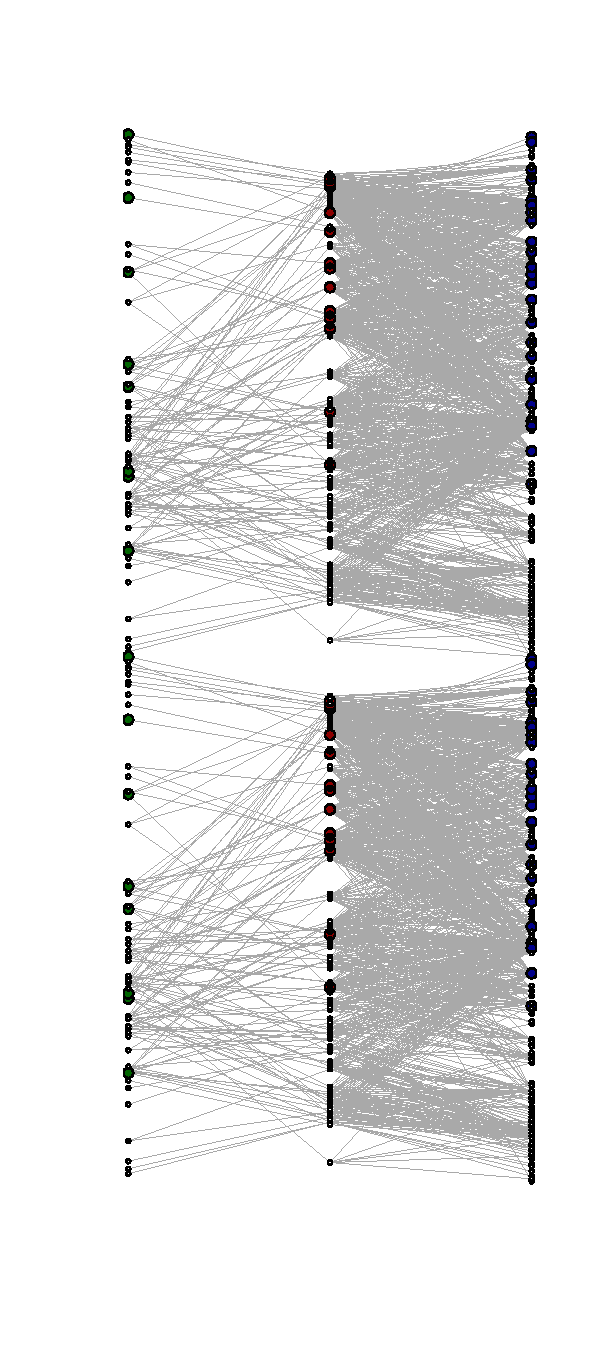
\includegraphics[width=0.5\textwidth]{figures/metaweb_sampling}
\end{figure}

\newpage

%------------------------
\subsection*{Figure 2}

\begin{figure}[ht!]
\centering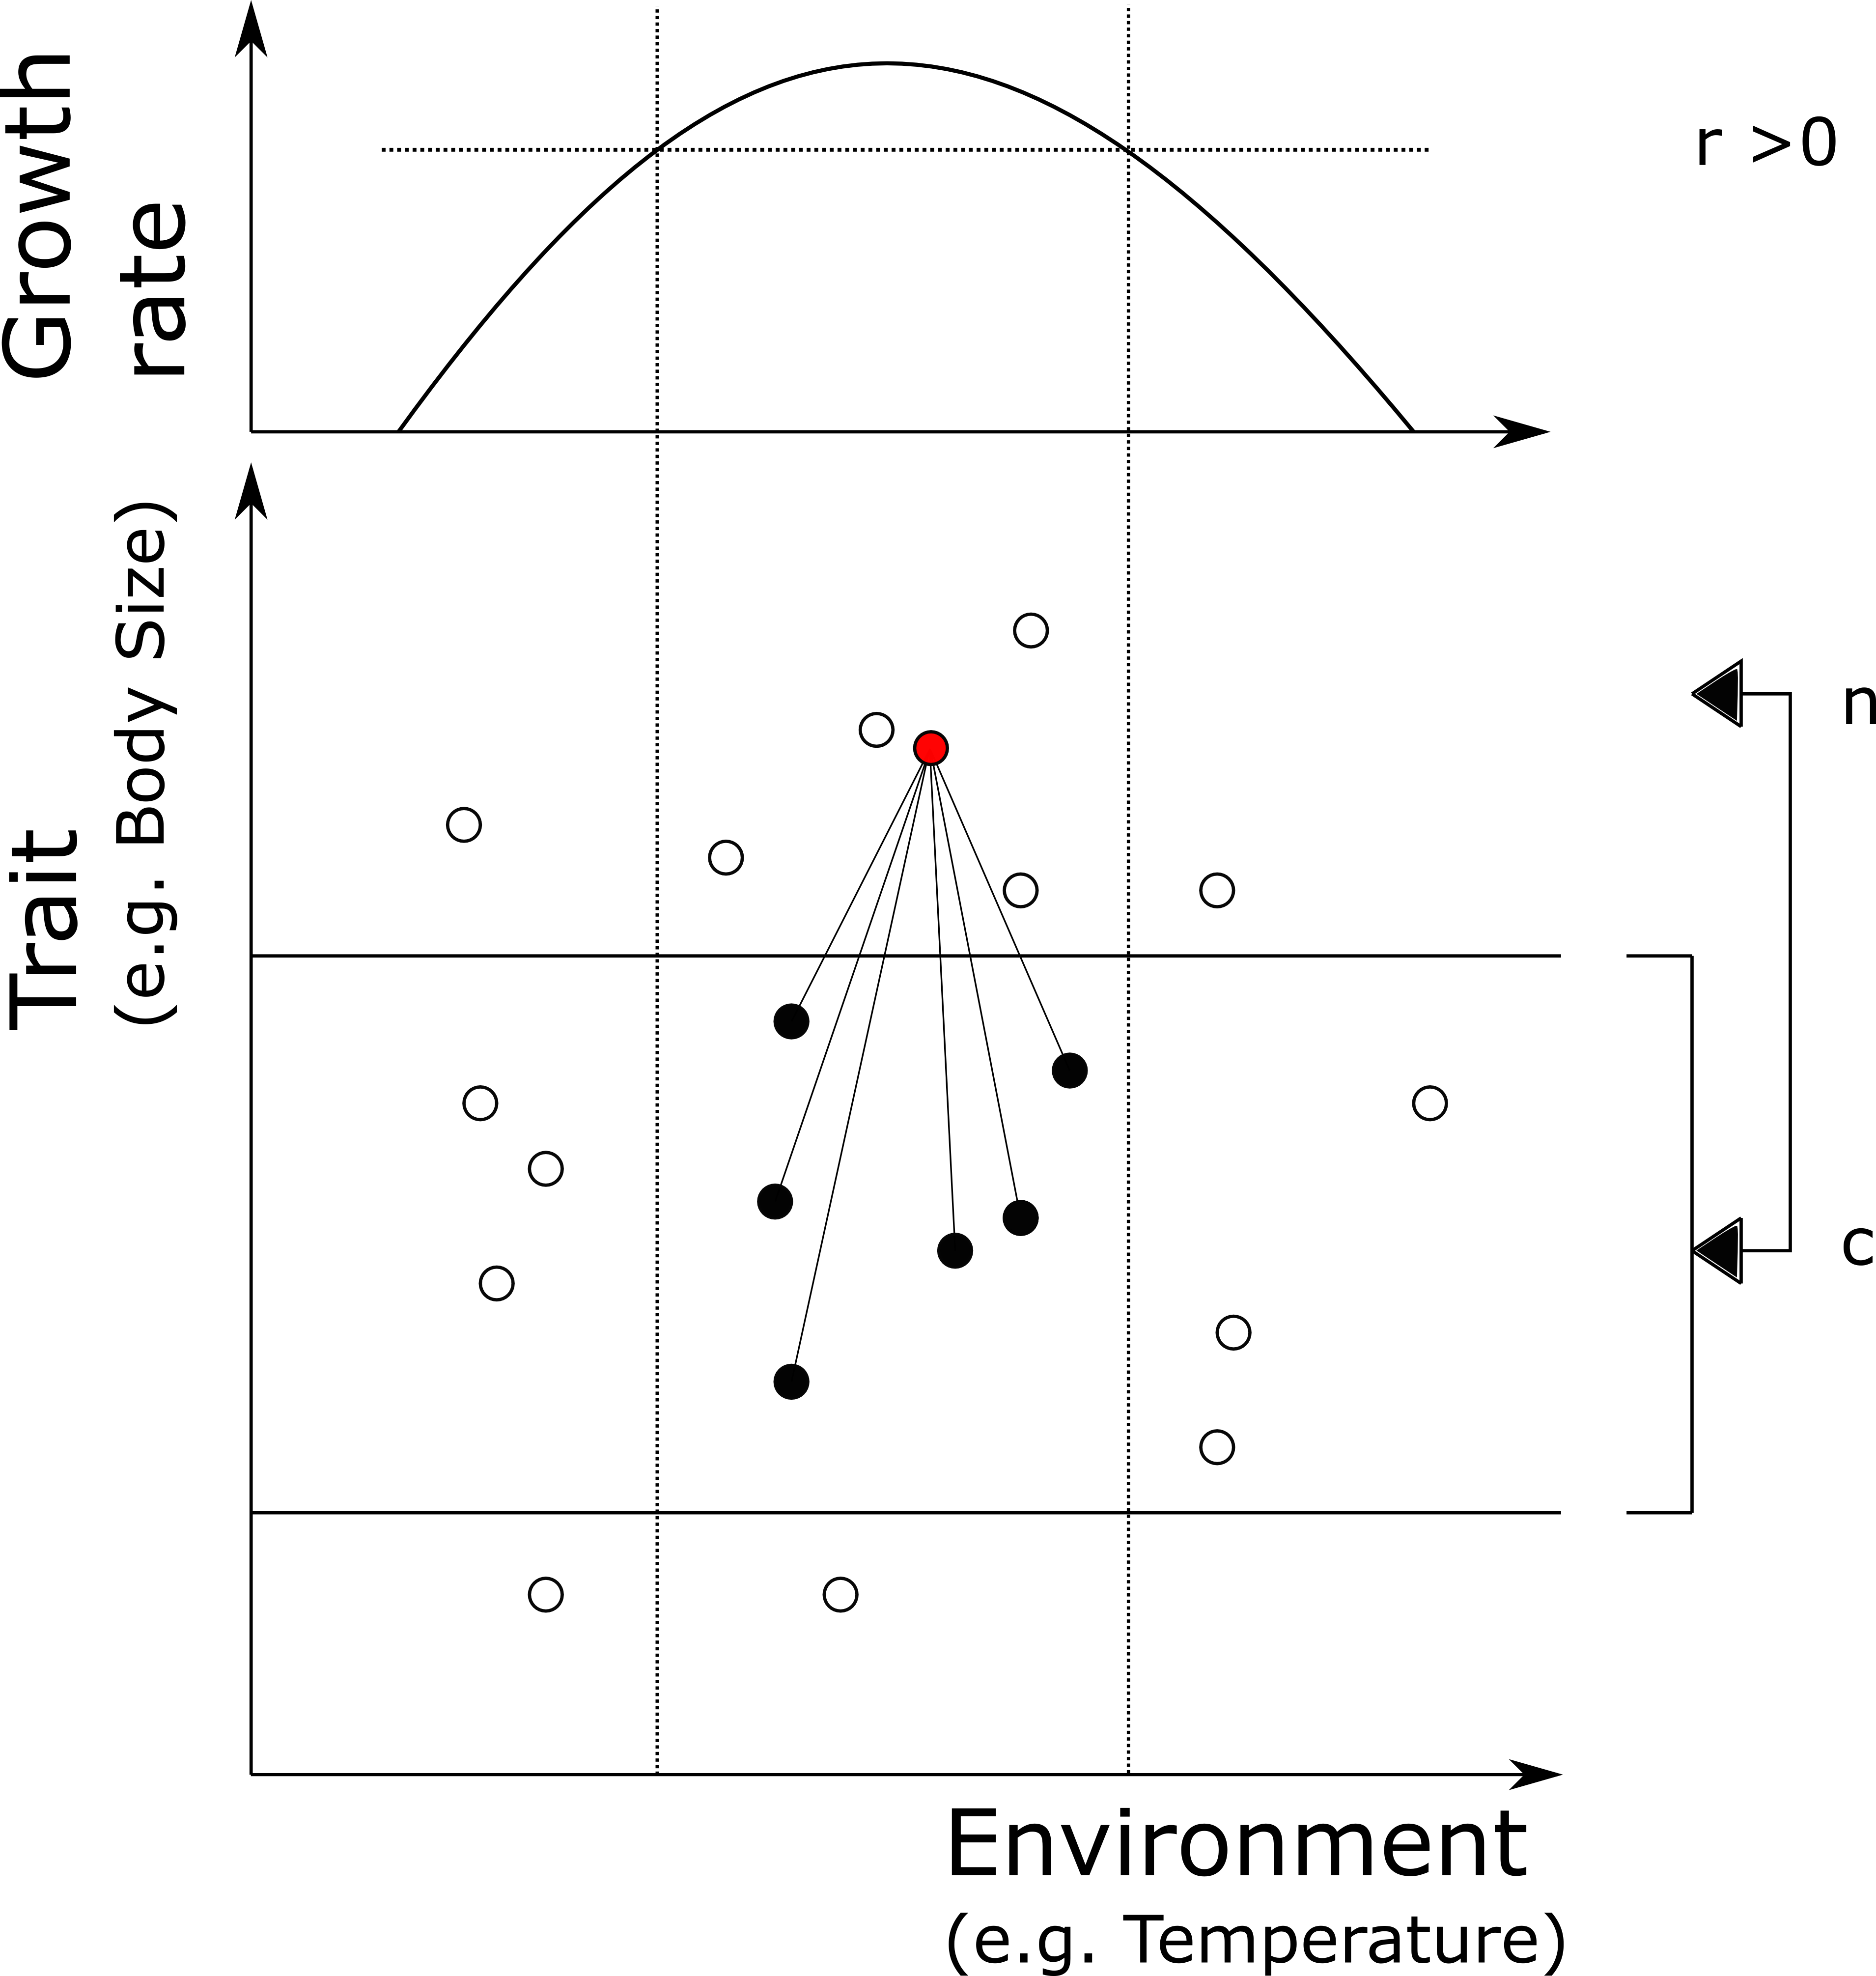
\includegraphics[width=0.6\textwidth]{figures/integrated_niche}
\end{figure}

\newpage

%------------------------
\subsection*{Figure 3}

\begin{figure}[ht!]
\centering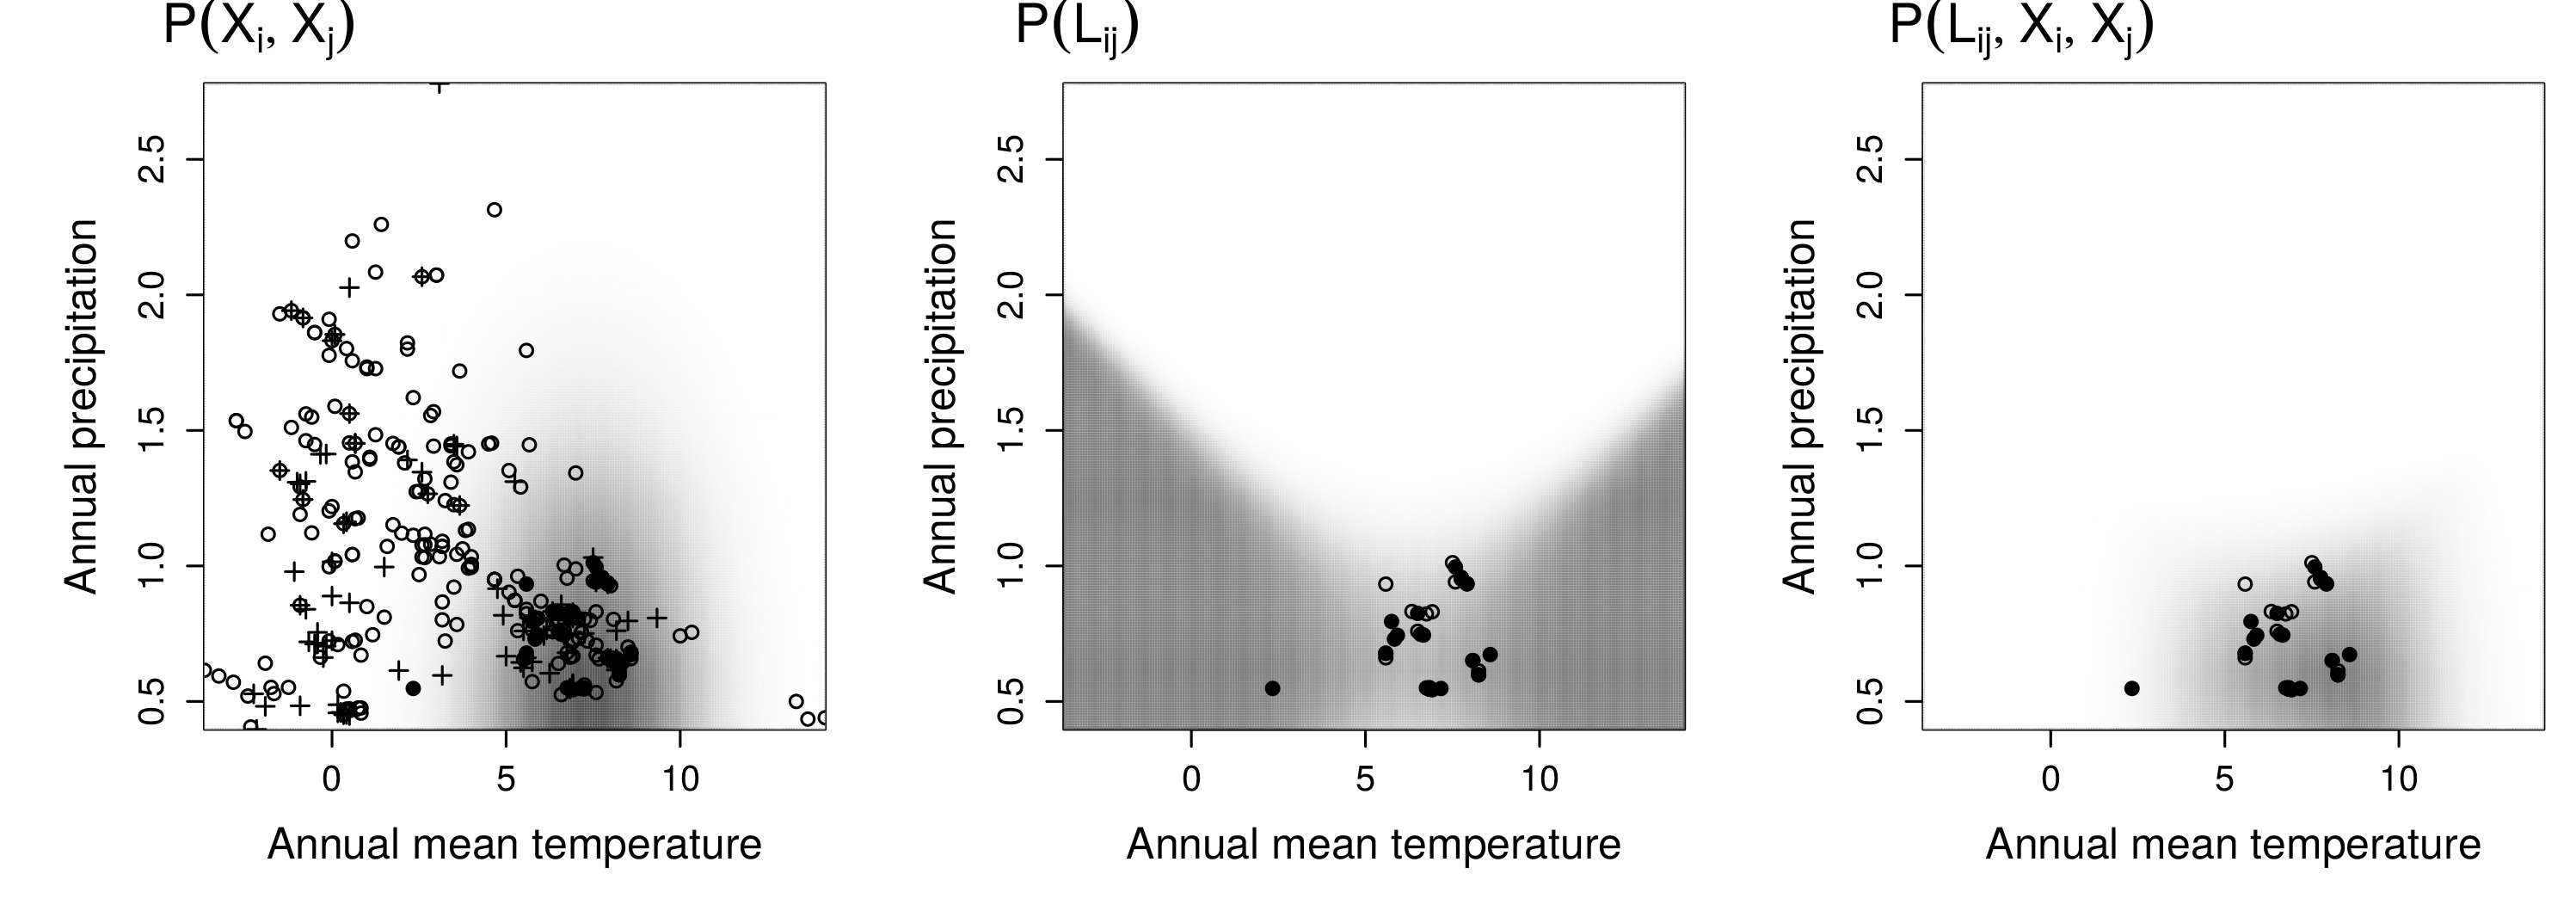
\includegraphics[width=0.8\textwidth]{figures/example_pair}
\end{figure}

\newpage

%------------------------
\subsection*{Figure 4}

\begin{figure}[ht!]
\centering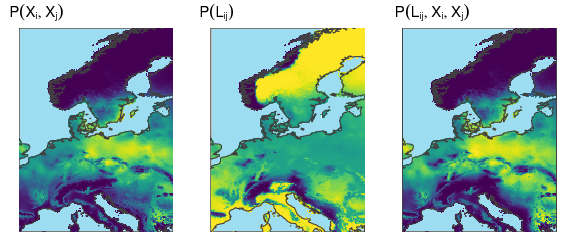
\includegraphics[width=0.8\textwidth]{figures/map_pair}
\end{figure}

\newpage

%------------------------
\subsection*{Figure 5}

\begin{figure}[ht!]
\centering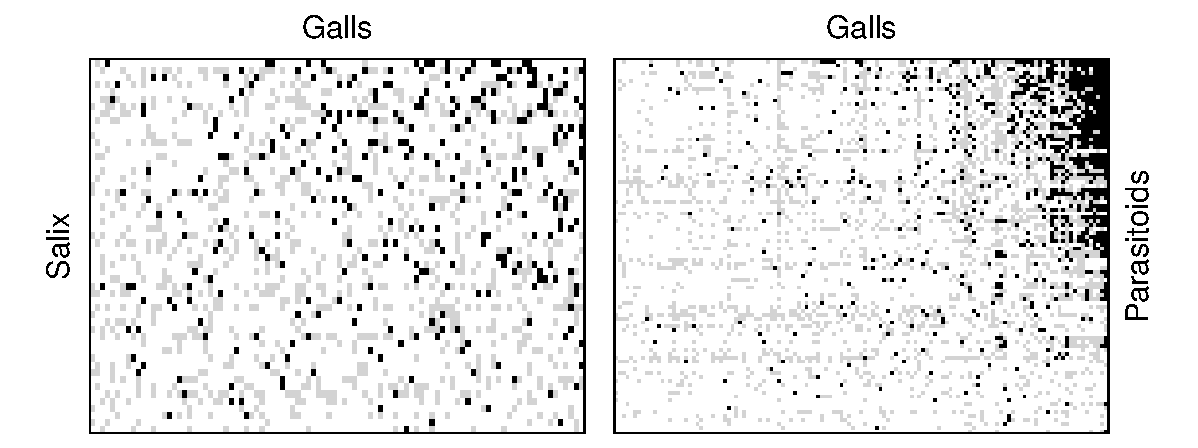
\includegraphics[width=0.8\textwidth]{figures/mw_holes}
\end{figure}

\newpage

%------------------------
\subsection*{Figure 6}

\begin{figure}[ht!]
\centering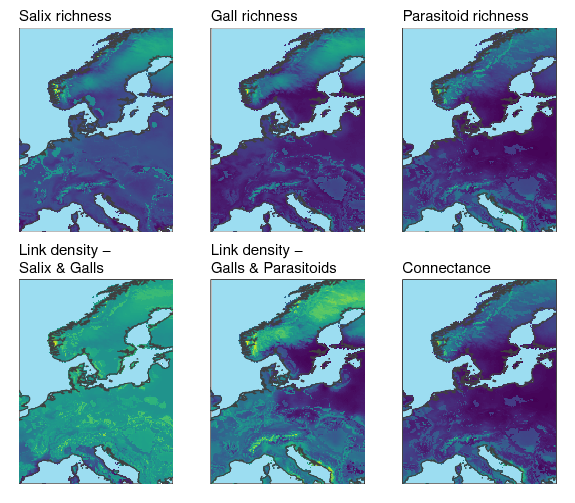
\includegraphics[width=0.8\textwidth]{figures/map_connectance}
\end{figure}

\newpage


%========================================================%
\end{document}
